\documentclass[tikz,border=8pt]{standalone}
\usetikzlibrary{arrows.meta,positioning}

\definecolor{maingreen}{HTML}{E8F5E9}
\definecolor{mainborder}{HTML}{2E7D32}
\definecolor{removeamber}{HTML}{FFF8E1}
\definecolor{removeborder}{HTML}{F9A825}
\definecolor{retrievalorange}{HTML}{FFF3E0}
\definecolor{retrievalborder}{HTML}{EF6C00}
\definecolor{finalblue}{HTML}{E3F2FD}
\definecolor{finalborder}{HTML}{1565C0}
\definecolor{stratapurple}{HTML}{F3E5F5}
\definecolor{strataborder}{HTML}{7B1FA2}
\definecolor{stagegrey}{HTML}{F1F5F9}
\definecolor{textdark}{HTML}{243B53}

\begin{document}
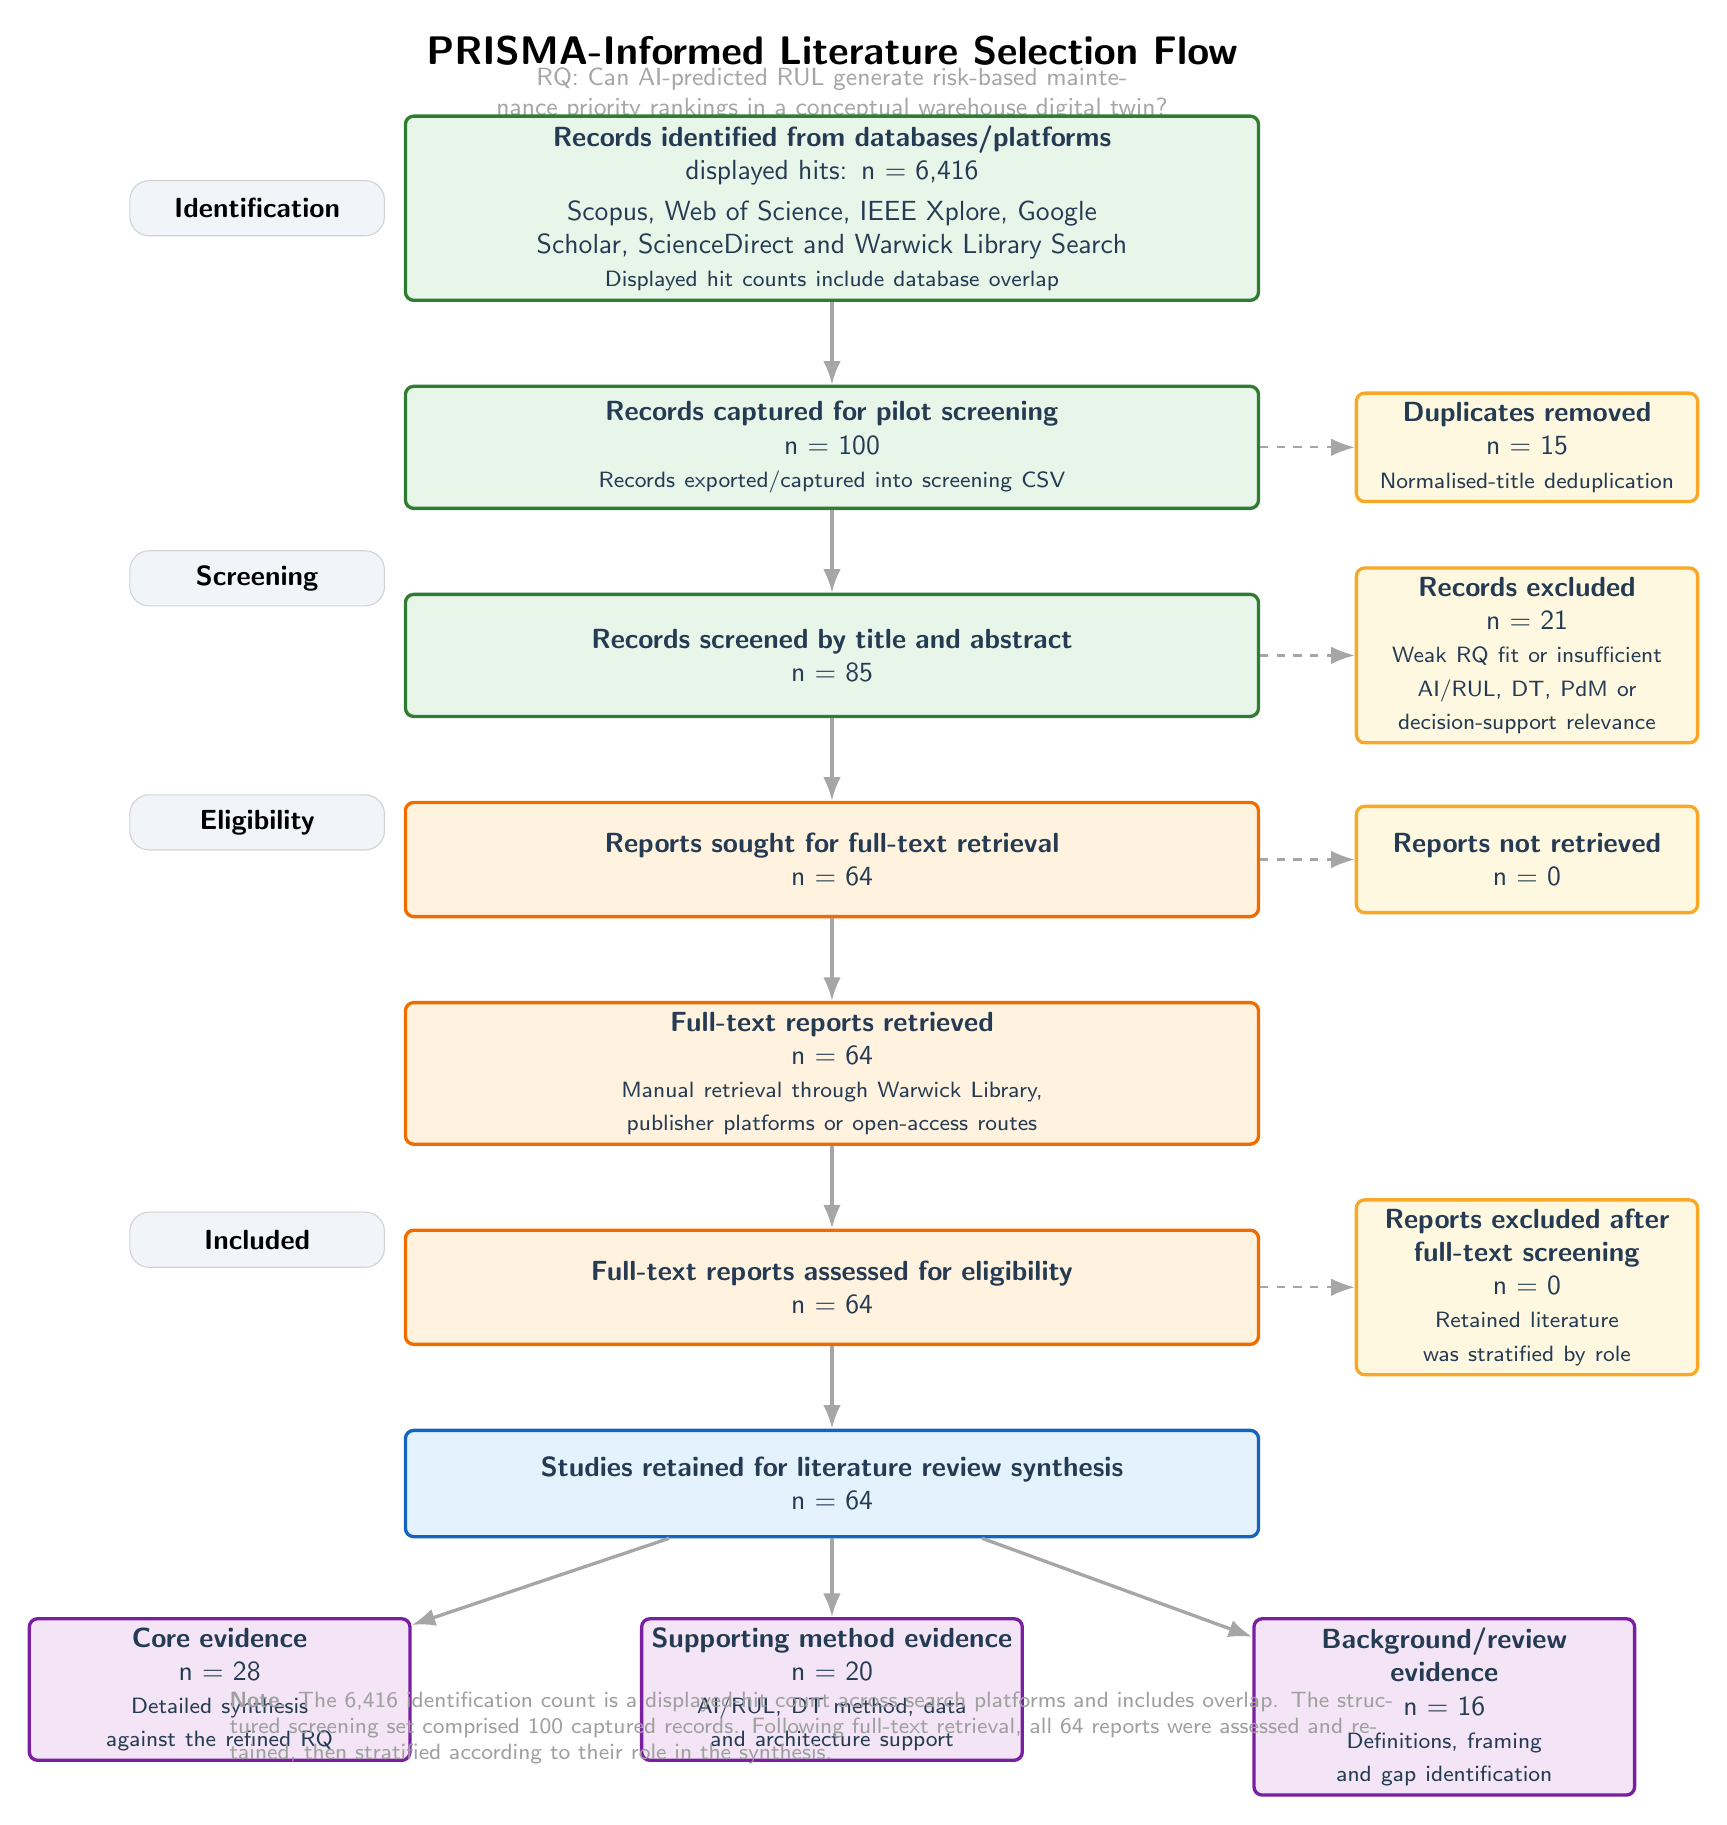
\begin{tikzpicture}[
  font=\sffamily,
  main/.style={rectangle, rounded corners=3pt, draw=mainborder, fill=maingreen, very thick, align=center, text width=10.6cm, minimum height=1.55cm, text=textdark},
  retrieval/.style={rectangle, rounded corners=3pt, draw=retrievalborder, fill=retrievalorange, very thick, align=center, text width=10.6cm, minimum height=1.45cm, text=textdark},
  removal/.style={rectangle, rounded corners=3pt, draw=removeborder, fill=removeamber, very thick, align=center, text width=4.1cm, minimum height=1.35cm, text=textdark},
  final/.style={rectangle, rounded corners=3pt, draw=finalborder, fill=finalblue, very thick, align=center, text width=10.6cm, minimum height=1.35cm, text=textdark},
  strata/.style={rectangle, rounded corners=3pt, draw=strataborder, fill=stratapurple, very thick, align=center, text width=4.6cm, minimum height=1.35cm, text=textdark},
  stage/.style={rectangle, rounded corners=7pt, draw=gray!35, fill=stagegrey, align=center, text width=3.0cm, minimum height=0.7cm, font=\sffamily\bfseries},
  arrow/.style={-{Latex[length=3mm]}, very thick, draw=gray!70},
  dasharrow/.style={-{Latex[length=3mm]}, thick, dashed, draw=gray!70},
  node distance=1.05cm
]

\node[align=center, font=\sffamily\bfseries\Large] at (0,1.1) {PRISMA-Informed Literature Selection Flow};
\node[align=center, font=\sffamily\small, text=gray!70, text width=15cm] at (0,0.55) {RQ: Can AI-predicted RUL generate risk-based maintenance priority rankings in a conceptual warehouse digital twin?};

\node[stage] at (-7.3,-0.9) {Identification};
\node[main] (identified) at (0,-0.9) {\textbf{Records identified from databases/platforms}\\
displayed hits: n = 6,416\\[1mm]
Scopus, Web of Science, IEEE Xplore, Google Scholar, ScienceDirect and Warwick Library Search\\
{\footnotesize Displayed hit counts include database overlap}};

\node[main, below=of identified] (captured) {\textbf{Records captured for pilot screening}\\
n = 100\\
{\footnotesize Records exported/captured into screening CSV}};
\node[removal, right=1.2cm of captured] (duplicates) {\textbf{Duplicates removed}\\
n = 15\\
{\footnotesize Normalised-title deduplication}};

\node[stage] at (-7.3,-5.6) {Screening};
\node[main, below=of captured] (screened) {\textbf{Records screened by title and abstract}\\
n = 85};
\node[removal, right=1.2cm of screened] (taex) {\textbf{Records excluded}\\
n = 21\\
{\footnotesize Weak RQ fit or insufficient AI/RUL, DT, PdM or decision-support relevance}};

\node[stage] at (-7.3,-8.7) {Eligibility};
\node[retrieval, below=of screened] (sought) {\textbf{Reports sought for full-text retrieval}\\
n = 64};
\node[removal, right=1.2cm of sought] (notret) {\textbf{Reports not retrieved}\\
n = 0};

\node[retrieval, below=of sought] (retrieved) {\textbf{Full-text reports retrieved}\\
n = 64\\
{\footnotesize Manual retrieval through Warwick Library, publisher platforms or open-access routes}};
\node[retrieval, below=of retrieved] (assessed) {\textbf{Full-text reports assessed for eligibility}\\
n = 64};
\node[removal, right=1.2cm of assessed] (ftex) {\textbf{Reports excluded after full-text screening}\\
n = 0\\
{\footnotesize Retained literature was stratified by role}};

\node[stage] at (-7.3,-14.0) {Included};
\node[final, below=of assessed] (included) {\textbf{Studies retained for literature review synthesis}\\
n = 64};

\node[strata, below left=1.0cm and -0.1cm of included] (core) {\textbf{Core evidence}\\
n = 28\\
{\footnotesize Detailed synthesis against the refined RQ}};
\node[strata, below=1.0cm of included] (support) {\textbf{Supporting method evidence}\\
n = 20\\
{\footnotesize AI/RUL, DT method, data and architecture support}};
\node[strata, below right=1.0cm and -0.1cm of included] (background) {\textbf{Background/review evidence}\\
n = 16\\
{\footnotesize Definitions, framing and gap identification}};

\draw[arrow] (identified) -- (captured);
\draw[dasharrow] (captured.east) -- (duplicates.west);
\draw[arrow] (captured) -- (screened);
\draw[dasharrow] (screened.east) -- (taex.west);
\draw[arrow] (screened) -- (sought);
\draw[dasharrow] (sought.east) -- (notret.west);
\draw[arrow] (sought) -- (retrieved);
\draw[arrow] (retrieved) -- (assessed);
\draw[dasharrow] (assessed.east) -- (ftex.west);
\draw[arrow] (assessed) -- (included);
\draw[arrow] (included) -- (core);
\draw[arrow] (included) -- (support);
\draw[arrow] (included) -- (background);

\node[align=left, text width=15.3cm, font=\sffamily\footnotesize, text=gray!75] at (0,-20.2) {
\textbf{Note.}
The 6,416 identification count is a displayed-hit count across search platforms and includes overlap.
The structured screening set comprised 100 captured records.
Following full-text retrieval, all 64 reports were assessed and retained, then stratified according to their role in the synthesis.
};

\end{tikzpicture}
\end{document}
